\documentclass[answers]{exam}
\usepackage{../MT2024}
\usepackage{graphicx}
\graphicspath{ {./images/} }

\title{Complex Analysis -- Sheet 1\\Complex differentiability, Branches}
\author{YOUR NAME HERE :)}
\date{Michaelmas Term 2024}
% accurate as of 18/10/2024


\begin{document}
\maketitle
\begin{questions}

\question%1
\begin{parts}
\part%1a
Let $f(z)=z e^{z}$. Write down expressions for the components $u(x, y), v(x, y)$, and check directly that $u$ is a harmonic function on $\mathbb{R}^{2}$.

\part%1b
Do the same for $f(z)=\sin z$, giving your expressions for $u$ and $v$ in terms of the hyperbolic functions $\sinh$, $\cosh$.
\end{parts}



\question%2
Suppose $f:U\to\mathbb C$ where $U=\{z:-\pi/2<\operatorname{Re}z<\pi/2\}$ and $f(z)=\sin z$. Consider a grid made of vertical lines $\{\operatorname{Re}z=\text{const}\}$ and horizontal intervals $\{\operatorname{Im}z=\text{const},\ -\pi/2<\operatorname{Re}z<\pi/2\}$. Describe $f(U)$ and sketch the image of this grid under $f$.



\question%3
Give an explicit $z \in \mathbb{C}$ such that $\sin z=2$.



\question%4
If $f: \mathbb{C} \to \mathbb{C}$ is a function, define $f^{\circ}(z):=\overline{f(\bar{z})}$. Show that $f$ is holomorphic if and only if $f^{\circ}$ is.



\question%5
Let $f: \mathbb{C} \to \mathbb{C}$ be the function defined by $f(x+i y)=\sqrt{|x||y|}$ for all $x, y \in \mathbb{R}$. Show that $f$ satisfies the Cauchy-Riemann equations at 0 but is not complex differentiable there.



\question%6
Suppose that $f=u+iv:\mathbb C\to\mathbb C$ is a holomorphic function and $u$ and $v$ are its real and imaginary parts. By writing $z$ in the polar coordinates $z=r\exp(i\theta)$ derive the polar version of the Cauchy-Riemann equations: \[
	\partial_ru=\frac1r\partial_\theta v,\qquad
	\partial_rv=-\frac1r\partial_\theta u.
\]



\question%7
Suppose that $f: \mathbb{C} \to \mathbb{C}$ is a holomorphic function. Show that if any one of the following conditions is satisfied then $f$ is constant:
\begin{parts}
\part%7a
$\operatorname{Re}(f)$ is constant;

\part%7b
$\operatorname{Im}(f)$ is constant;

\part%7c
$|f|$ is constant.
\end{parts}



\question%8
Show that the series $\sum_{n=1}^{\infty} \frac{z^{n}}{n}$ has radius of convergence 1. Let $f(z)$ be the function to which it converges on the domain $D=\{z \in \mathbb{C}:|z|<1\}$. Show that $\exp (f(z))=\frac{1}{1-z}$.



\question%9
\begin{parts}
\part%9a
Suppose that $l(z)$ is holomorphic on $\mathbb C\setminus(-\infty,0]$ and satisfies $\exp l(z)=z$. Show that \[
	l(z)=\operatorname{Log}(z)+2n\pi i
\] for some $n\in\mathbb Z$ where $\operatorname{Log}(z)$ is the holomorphic branch of $[\log]$ defined in lectures.

\part%9b
Show that there is no holomorphic function $\lambda(z)$ on $\mathbb C\setminus\{0\}$ such that $\exp\lambda(z)=z$.
\end{parts}



\question%10
Consider a domain $\mathbb C\setminus\gamma$ where $\gamma$ is a curve from the figure below. There is a unique branch of the argument such that its value at $a$ is 0. Determine the argument of $b$, $c$, $d$, and $e$.
\begin{center}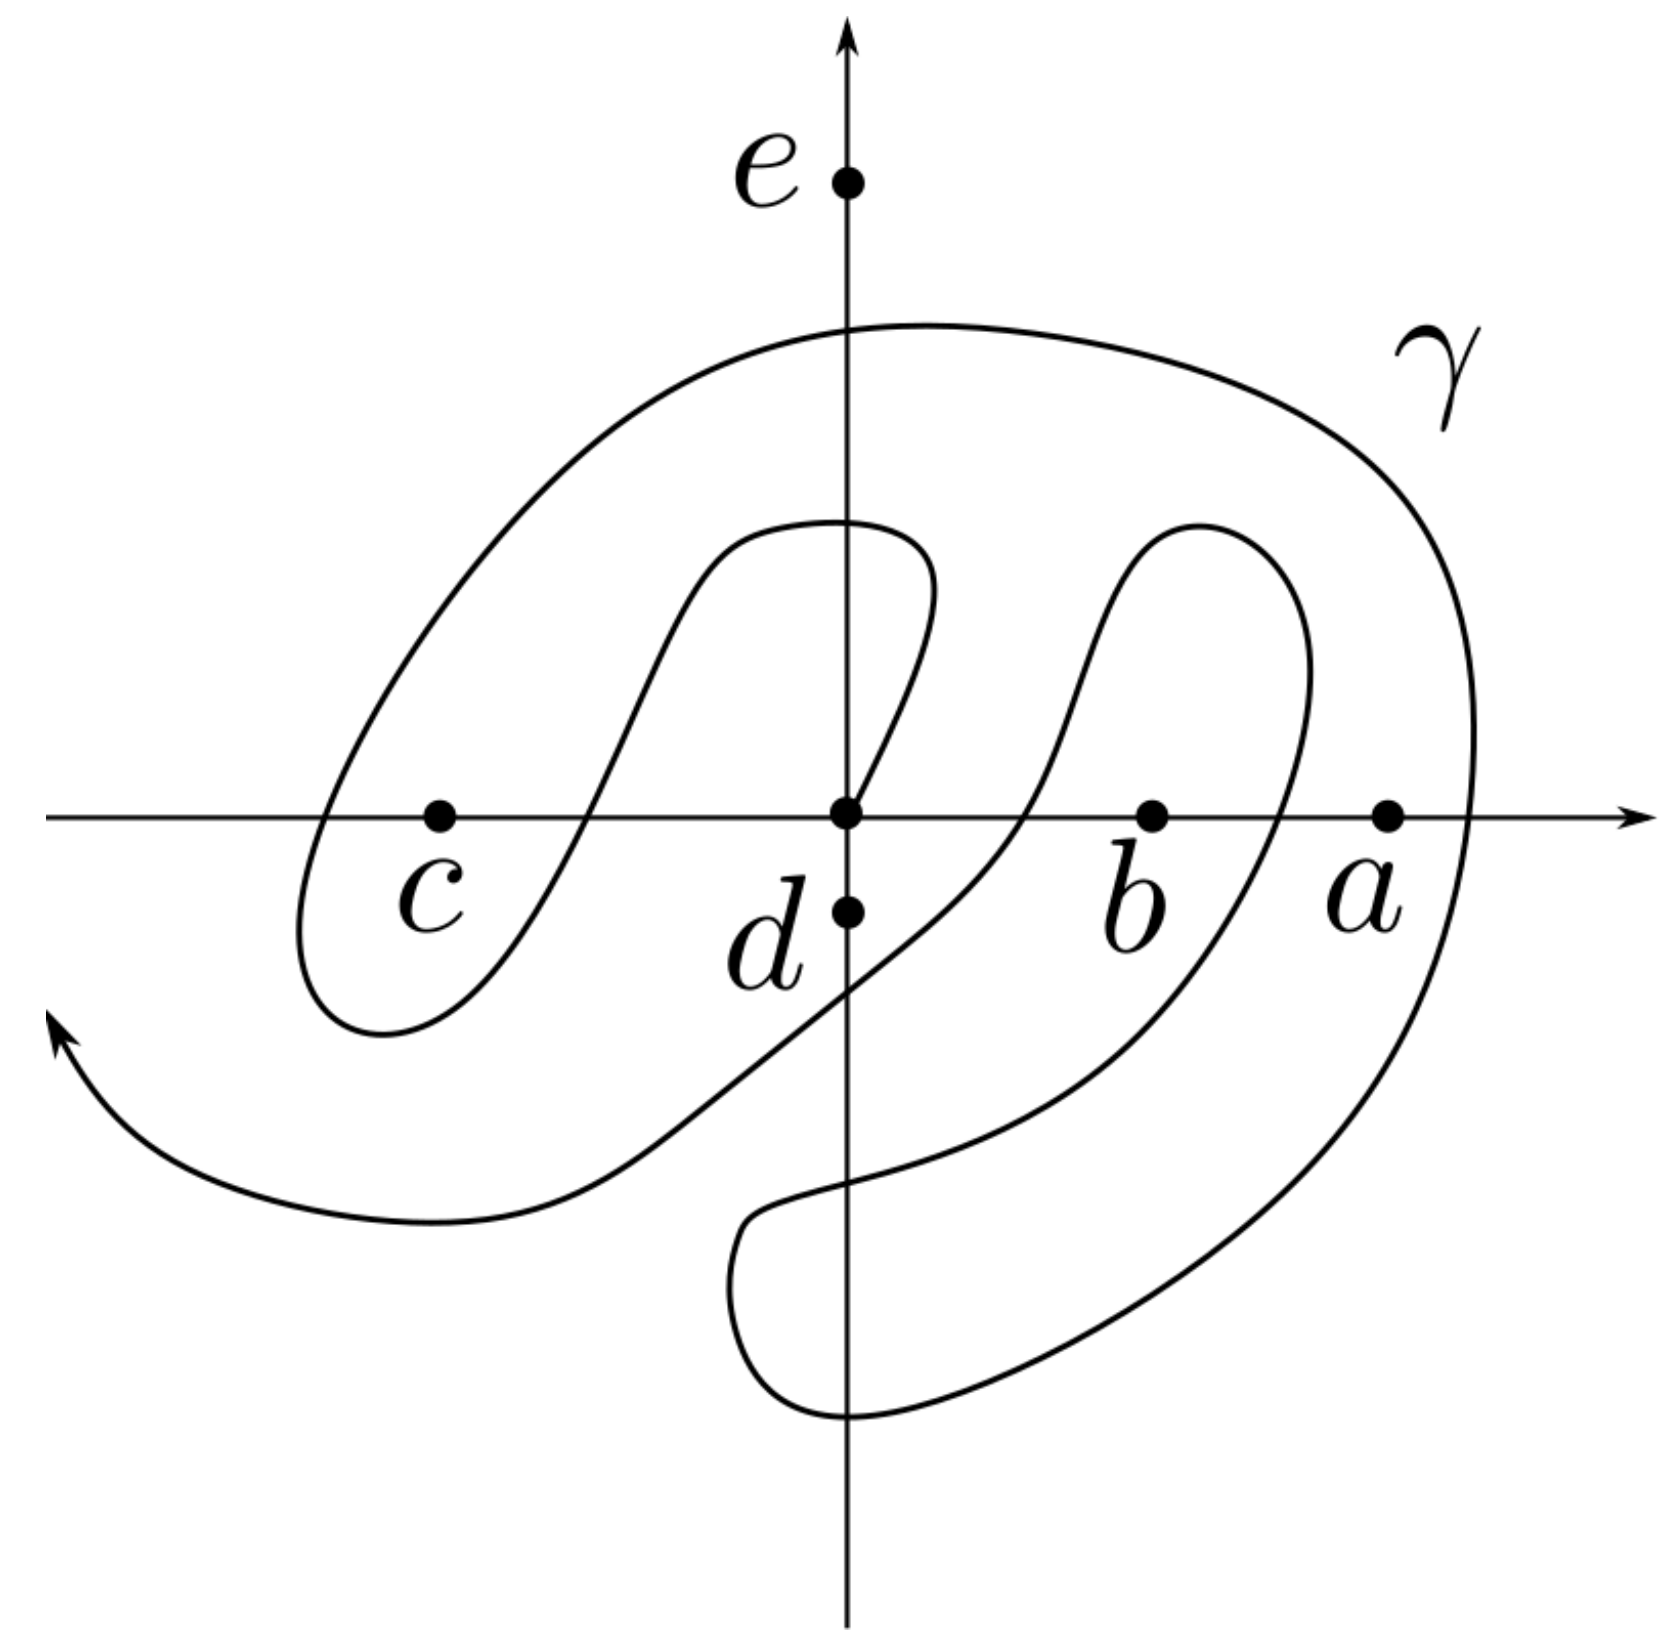
\includegraphics[width=7cm]{sheet 1 q 10}\end{center}



\question%11
There are unique holomorphic branches of $\log z, \sqrt{z}$ and $\sqrt[3]{z}$ on the cut plane $\mathbb{C} \setminus\{\text{negative imaginary axis}\}$ such that $\log 1=0; \sqrt{1}=1; \sqrt[3]{1}=1$. For these branches determine \[
	\log (1+i), \qquad \sqrt{-1-i}, \qquad \sqrt[3]{-2}, \qquad \sqrt{1-i}.
\]



\question%12 one of them is real (around 0.2) which is kind of funny
Determine all values of $i^i$.



\question%13
Prove the following statement that is known as Lucas or Gauss-Lucas theorem. Let $f$ be a non-constant polynomial with complex coefficients. Then all zeros of $f'$ lie in the convex hull of zeros of $f$. [\emph{Hint: you might first try to prove that if all zeros of $f$ have positive imaginary part, then the same is true for all zeros of $f'$.}]



\question%14
\begin{parts}
\part%14a
Prove the following statement known as Pringsheim or Vivanti–Pringsheim theorem. Let $f$ be defined by a power series $\sum a_nz^n$ such that all coefficients are real and non-negative and the radius of convergence is 1. Show that $z=1$ is a singular point of $f$. Namely, there is no function which is holomorphic in a neighbourhood of 1 and coincides with $f$ inside the unit disc. You can assume that if $f$ is not singular at 1 then $f$ has a power series expansion around any point $x\in[0,1)$ with the radius of convergence strictly larger than $1-x$.\\\relax[\emph{Note that being singular on the boundary and the divergence of the series are not the same thing. For example, if $f(z)=\sum z^n$, then $f=1/(1-z)$ which is holomorphic everywhere except $z = 1$. So $z = 1$ is the only singular point but the
series diverges for every $z$ with $|z| = 1$.}]

\part%14b
Show that there is a function which is holomorphic in $\mathbb D$ but has no analytic extension, namely there is no large domain and a holomorphic function there which coincides with $f$ in $\mathbb D$.
\end{parts}

\end{questions}

\end{document}
